\section{Analysis of the EDSLs}
\label{sec:analysis-of-the-edsls}
    \frame{\sectionpage}

    \subsection{Lava}
    \label{subsec:lava}
        % Lava intro
        \begin{frame}
            \frametitle{Lava}

            \begin{itemize}
                \item Developed at Chalmers University of Technology, Sweden
                    \begin{itemize}
                        \item Initially by Koen Claessen and Mary Sheeran
                        \item Later also Per Bjesse and David Sands
                    \end{itemize}

                \item Has several \emph{dialects}
                    \begin{itemize}
                        \item \texttt{chalmers-lava}, \texttt{xilinx-lava}, \texttt{kansas-lava}, etc. 
                        \item We focus on the ``canonical'' \texttt{chalmers-lava}
                    \end{itemize}
            \end{itemize}
        \end{frame}

        \begin{frame}
            \frametitle{Lava's \emph{key} characteristics}

            \begin{itemize}
                \item Deep-embedded
                \item Observable sharing
                    \begin{itemize}
                        \item ``Type-safe pointer equality'' to detect sharing and recursion
                        \item Advantages and disadvantages clearer with examples
                    \end{itemize}
                \item Capable of simulation, verification and synthesis
                    \begin{itemize}
                        \item Generates \emph{flat} VHDL
                        \item External tools for verification
                    \end{itemize}
                \item Very ``functional'' style of hardware description
                    \begin{itemize}
                        \item Will become clearer with examples
                    \end{itemize}
            \end{itemize}
        \end{frame}

        \begin{frame}
            \frametitle{Lava: Adders}
            \haskellfile{code/lava-adders.hs}
        \end{frame}

        \begin{frame}
            \frametitle{Lava: Simulation and verification}

            \begin{itemize}
                \item A taste of simulation in Lava:
                    \haskellfile{code/lava-simulation-halfadder.hs}
                    \begin{itemize}
                        \item Cannot be easily automated: equality of \texttt{Signal} is non-trivial
                    \end{itemize}

                \item And verification\ldots
                    \haskellfile{code/lava-verify-fulladder-comm.hs}
                    \begin{itemize}
                        \item Advantage: Used in conjunction with an external SAT solver (e.g. \emph{Satzoo})
                        \item Disadvantage: Only verifies instances of \emph{specific size}
                    \end{itemize}
            \end{itemize}
        \end{frame}

        % Lava ALU
        \begin{frame}
            \frametitle{Lava: ALU}
            \haskellfile{code/lava-alu.hs}
        \end{frame}

        \begin{frame}
            \frametitle{Remarks}

            \begin{itemize}
                \item Cannot introduce new, meaningful datatypes
                    \begin{itemize}
                        \item Only \texttt{Signal Bool} is synthesizable
                        \item Or tuples/lists thereof
                    \end{itemize}
                \item Input/Output types have to be \emph{uncurried}
                \item Weak type-safety over the inputs/outputs
                    \begin{itemize}
                        \item Working with tuples is tiresome and has limitations
                        \item Lists don't enforce \emph{size} constraints
                    \end{itemize}
            \end{itemize}
        \end{frame}

        % Lava RAM64
        \begin{frame}
            \frametitle{Lava: RAM64}
            \haskellfile{code/lava-ram64.hs}
        \end{frame}

        \begin{frame}
            \frametitle{Remarks}

            \par{Positive:}
            \begin{itemize}
                \item Uses host language for binding (\texttt{let}/\texttt{where}) and recursion
                \item Uses host language for structural combinators
            \end{itemize}

            \par{Negative:}
            \begin{itemize}
                \item Again, weak type-safety of lists
                    \begin{itemize}
                        \item Extra \texttt{Int} parameter controls port \emph{sizes}
                    \end{itemize}
                \item \emph{No modularity} in the generated VHDL code.
            \end{itemize}
        \end{frame}

        % Lava CPU
        \begin{frame}
            \frametitle{Lava: \emph{Hack} CPU (some parts)}
            \haskellfile{code/lava-cpu.hs}
        \end{frame}

        \begin{frame}
            \frametitle{Remarks}

            \par{Could benefit from:}
            \begin{itemize}
                \item Fixed-length vectors
                    \begin{itemize}
                        \item ForSyDe-style or with type-level naturals in recent GHC.
                    \end{itemize}
                \item Slicing operators over vectors
                \item \emph{Synthesizable} user-defined datatypes
            \end{itemize}
        \end{frame}


    \subsection{ForSyDe}
    \label{subsec:forsyde}
        % ForSyDe intro
        \begin{frame}
            \frametitle{ForSyDe}

            \begin{itemize}
                \item Based on the ``Formal System Design'' approach
                    \begin{itemize}
                        \item Royal Institute of Technology - KTH, Sweden
                    \end{itemize}
                \item Available for Haskell and SystemC
                \item Has BOTH shallow and deep-embedded ``versions''
                    \begin{itemize}
                        \item Same library, subtle distinction
                        \item Will become clearer with examples
                    \end{itemize}
                \item \emph{Template Haskell} to express circuits with Haskell syntax
            \end{itemize}
        \end{frame}

        \begin{frame}
            \frametitle{ForSyDe's key concepts}

            \begin{itemize}
                \item Models of Computation (MoCs)
                    \begin{itemize}
                        \item We focus on the \emph{synchronous} MoC
                    \end{itemize}
                \item Processes
                    \begin{itemize}
                        \item A process belongs to a MoC
                        \item Built with a \emph{process constructor}
                    \end{itemize}
                \item Signals
                    \begin{itemize}
                        \item Connections among processes
                    \end{itemize}
            \end{itemize}
        \end{frame}

        \begin{frame}
            \frametitle{ForSyDe's key concepts}
            \begin{figure}[h!]
                \centerline{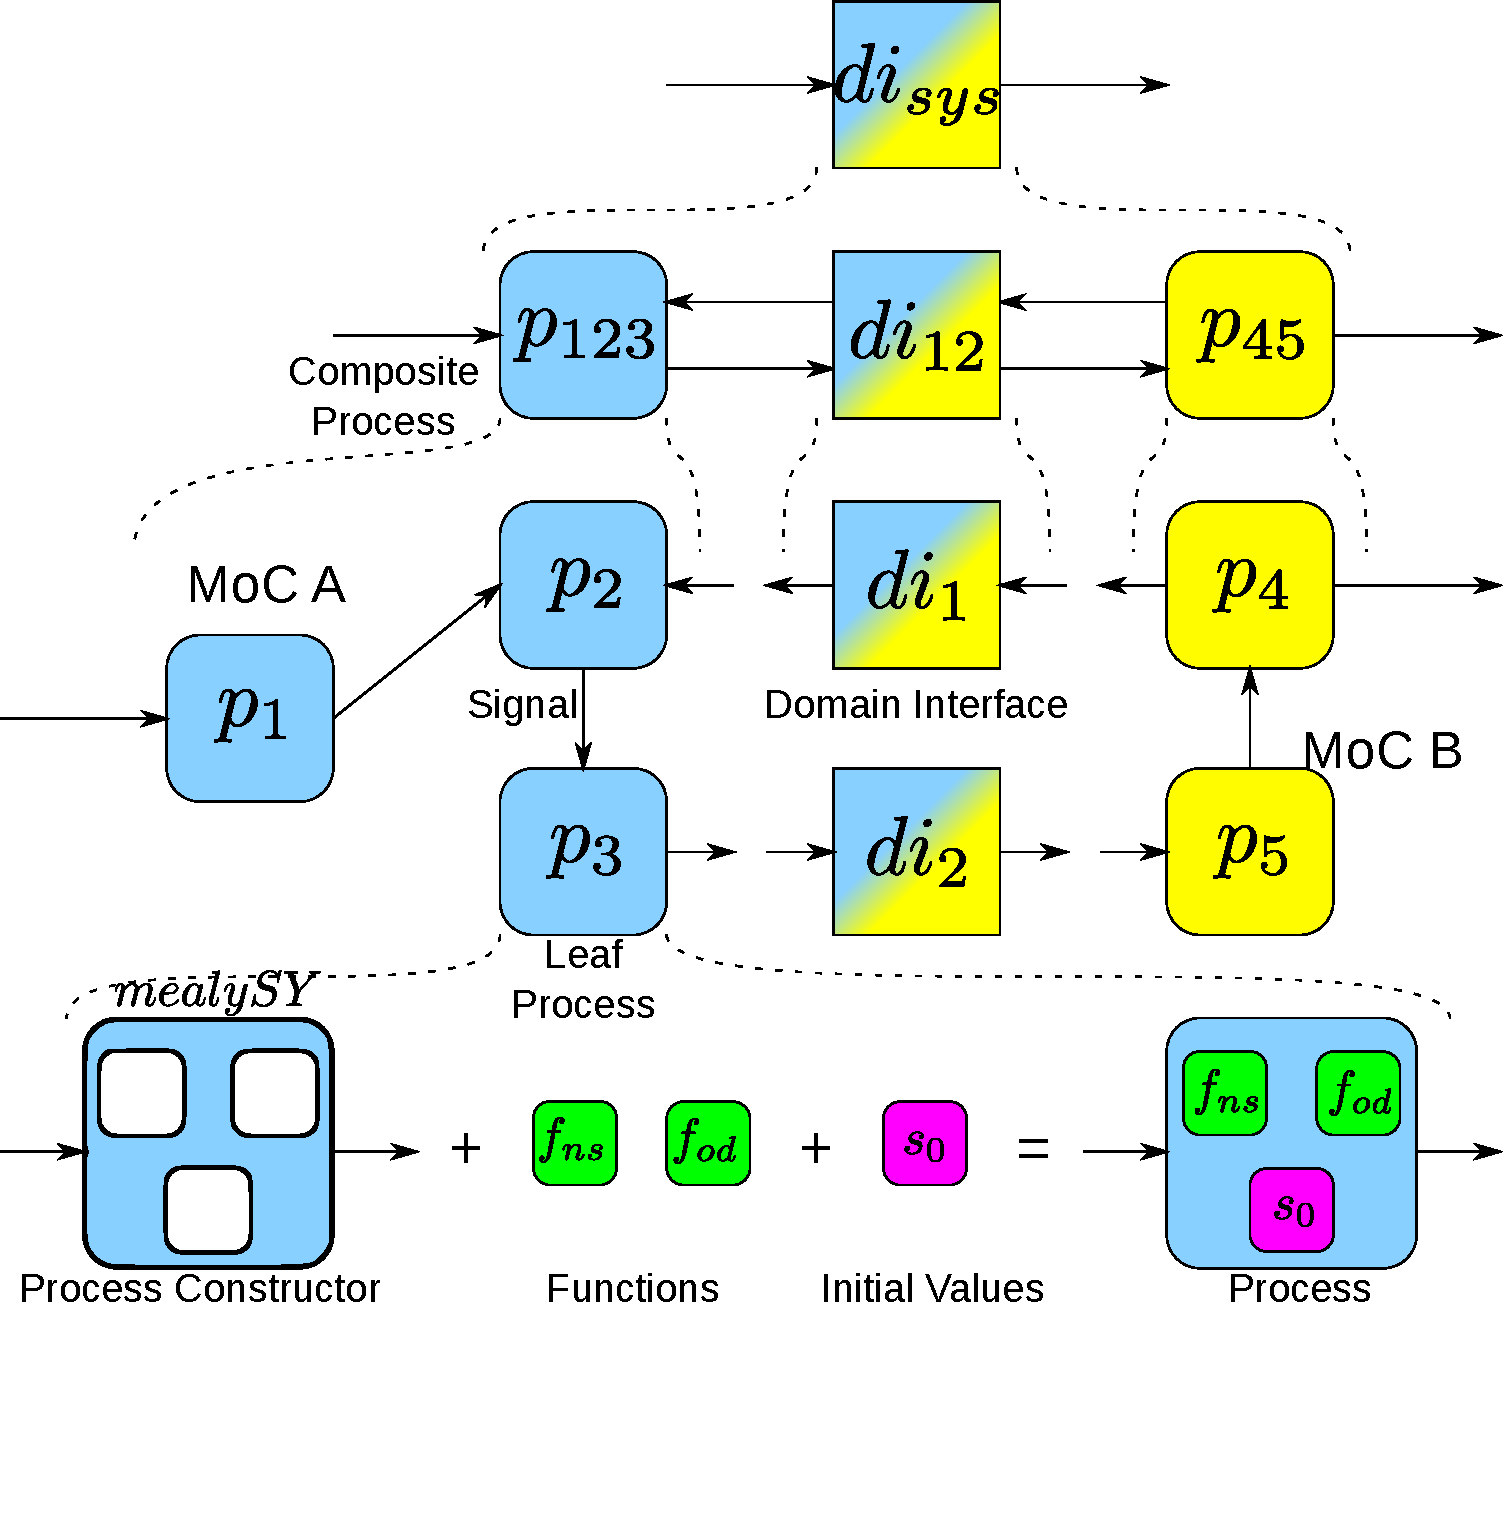
\includegraphics[width=0.8\textwidth]{imgs/forsyde-model.pdf}}
                \caption{Key concepts of the ForSyDe EDSL
                    \label{fig:forsyde-model}}
            \end{figure}
        \end{frame}

        % ForSyDe ALU non-synth
        \begin{frame}
            \frametitle{ForSyDe: ALU (non-synth)}
            \haskellfile{code/forsyde-alusim-slide1.hs}
        \end{frame}

        \begin{frame}
            \frametitle{ForSyDe: ALU (non-synth)}
            \haskellfile{code/forsyde-alusim-slide2.hs}
        \end{frame}

        \begin{frame}
            \frametitle{ForSyDe: synthesis restrictions}
            \par{Restrictions imposed on a model by ForSyDe so that it can be translated to VHDL:}
            \begin{itemize}
                \item ProcFun-related:
                    \begin{itemize}
                        \item Limited argument types (instances of \texttt{ProcType})
                        \item \texttt{Int}, \texttt{Int8}, \ldots, \texttt{Bool}, \texttt{Bit}
                        \item Enumerated types (deriving \texttt{Data} and \texttt{Lift})
                        \item Tuples and \texttt{FSVec}'s
                    \end{itemize}
                \item VHDL engine-related:
                    \begin{itemize}
                        \item No point-free notation
                        \item Single clause / no pattern matching
                        \item No \texttt{where} or \texttt{let} bindings
                    \end{itemize}
            \end{itemize}
        \end{frame}

        % ForSyDe ALU synth
        \begin{frame}
            \frametitle{ForSyDe: ALU (synthesizable)}
            \haskellfile{code/forsyde-alusyn-slide1.hs}
        \end{frame}

        \begin{frame}
            \frametitle{ForSyDe: ALU (synthesizable)}
            \haskellfile{code/forsyde-alusyn-slide2.hs}
        \end{frame}

        % ForSyDe Simulation

        % ForSyDe RAM64
        \begin{frame}
            \frametitle{ForSyDe: Muxes}
            \haskellfile{code/forsyde-muxes.hs}
        \end{frame}

        \begin{frame}
            \frametitle{Remarks}
            %% both advantage and disadvantage of ForSyDe
            \par{Positive:}
            \begin{itemize}
                \item Generated VHDL is very \emph{modular}
                    \begin{itemize}
                        \item One VHDL \emph{entity} per ForSyDe component
                        \item Good for tool integration
                    \end{itemize}
            \end{itemize}

            \par{Negative:}
            \begin{itemize}
                \item Interface ``conflicts'' caused by \texttt{FSVec} and process constructors
                    \begin{itemize}
                        \item ``zip-unzip'' pattern
                    \end{itemize}
            \end{itemize}
        \end{frame}

        \begin{frame}
            \frametitle{ForSyDe: RAM64}
            \haskellfile{code/forsyde-ram64.hs}
        \end{frame}

        \begin{frame}
            \frametitle{Remarks}

            \begin{itemize}
                \item Component \emph{instantiation}
                    \begin{itemize}
                        \item Introduces \emph{hierarchy} in the design
                        \item Influences generated VHDL
                    \end{itemize}
                \item \emph{Manual} name management
                    \begin{itemize}
                        \item Error-prone
                        \item Every process must have a \emph{unique} identifier
                        \item Already was a (lesser) issue with the muxes
                    \end{itemize}
            \end{itemize}
        \end{frame}

        % ForSyDe CPU
        \begin{frame}
            \frametitle{ForSyDe: \emph{Hack} CPU (part)}
            \haskellfile{code/forsyde-cpu-decoder.hs}
        \end{frame}


    \subsection{Coquet}
    \label{subsec:coquet}
        \begin{frame}
            \frametitle{The \texttt{Circuit} type}
            \coqfile{code/coquet-circuit-type.v}
        \end{frame}

        \begin{frame}
            \frametitle{Coquet}
            \coqfile{code/coquet-halfadder.v}
        \end{frame}

        \begin{frame}
            \frametitle{Coquet}
            \coqfile{code/coquet-fulladder.v}
        \end{frame}

        % Meaning relation
        \begin{frame}
            \frametitle{Coquet: Meaning relation}
            \coqfile{code/coquet-meaning-relation.v}
        \end{frame}

        % Specification definitions
        \begin{frame}
            \frametitle{Coquet: Specification}
            \coqfile{code/coquet-realise-implement.v}
        \end{frame}

        % Adder proof (1)
        \begin{frame}
            \frametitle{Coquet: Correctness proofs}
            \coqfile{code/coquet-halfadder-proof.v}
        \end{frame}

        % How to do proofs in Coquet (tac, etc)
        \begin{frame}
            \frametitle{Coquet: How to prove correctness}
            \coqfile{code/coquet-tac.v}
            % rinvert: invert derivation of meaning relation, following structure of circuit.
            % realise_all: use the Implement and Realise classes as hints to transform goals.
            % unreify_all: get rid of iso's
            % destruct all boolean, then proof by case analysis, not so important.
        \end{frame}
        % Adder proof (2)
